\documentclass{standalone}
  \usepackage{xeCJK}
  \usepackage{tikz}
  \usetikzlibrary{shapes.geometric, arrows.meta}
  
\begin{document}
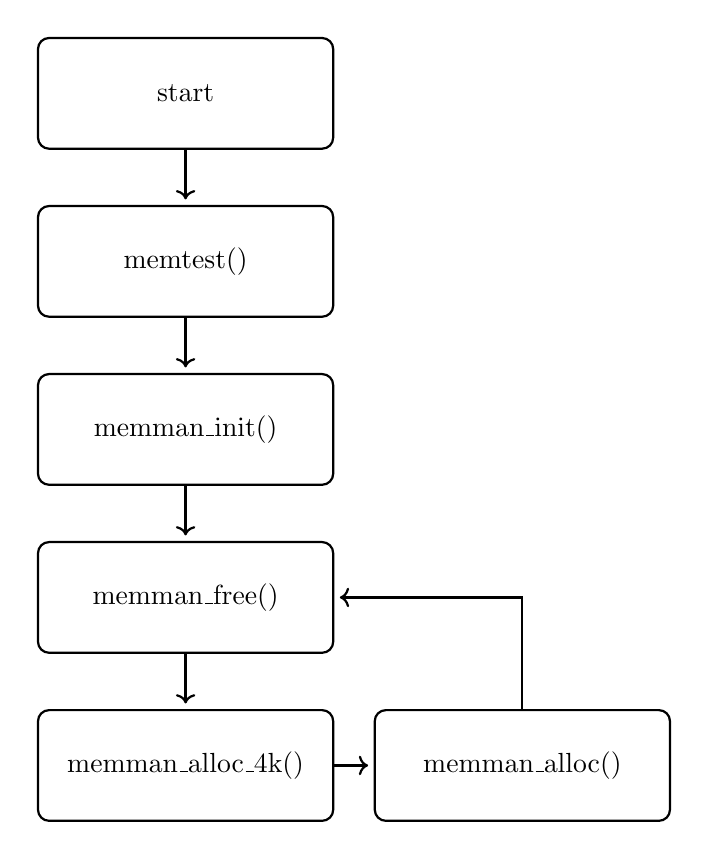
\begin{tikzpicture}
  [auto,
  block/.style={rectangle, draw=black, thick,
  text width=10em,align=center, rounded corners,
  minimum height=4em},
  line/.style={draw, thick, shorten >=2pt, ->}]

  \matrix [column sep=5mm,row sep=7mm]
  {
    \node [block] (start) {start}; & \\
    \node [block](test){memtest()}; & \\
    \node [block](init){memman\_init()}; & \\
    \node [block](free){memman\_free()}; & \\
    \node [block](alloc4k){memman\_alloc\_4k()}; & 
    \node [block](alloc){memman\_alloc()}; \\
  };
  \begin{scope}[every path/.style=line]
    \path (start) -- (test);
    \path (test) -- (init);
    \path (init) -- (free);
    \path (free) -- (alloc4k);
    \path (alloc4k) -- (alloc);
    \path (alloc) |- (free);
  \end{scope}
\end{tikzpicture}

\end{document}

%%% Local Variables:
%%% mode: latex
%%% TeX-master: t
%%% End:
